%\documentclass[11pt]{article}

\usepackage{mathtools}
\usepackage{color}
\usepackage{stmaryrd}
\usepackage{biblatex}
\usepackage{tikz}
\usepackage{wasysym}
\addbibresource{codigoscorrectores/bibliografia.bib}
\newtheorem{definition}{Definition}[section]
\newtheorem{lemma}{Definition}[section]
\newtheorem{example}{Definition}[section]
\newtheorem{theorem}{Definition}[section]
\DeclareMathOperator{\tr}{Tr}
\DeclareMathOperator{\diag}{Diag}
\newcommand{\matr}[1]{\mathbf{#1}}
\providecommand{\tq}{\mid}
\providecommand{\N}{\mathbb{N}}
\providecommand{\Z}{\mathbb{Z}}
\providecommand{\Q}{\mathbb{Q}}
\providecommand{\R}{\mathbb{R}}
\providecommand{\C}{\mathbb{C}}
\providecommand{\H}{\mathcal{H}}
\providecommand{\Im}[1]{Im(#1)}
\providecommand{\Re}[1]{Re(#1)}
\let\oldforall\forall
\renewcommand{\forall}{\oldforall\,}
\let\oldexists\exists
\renewcommand{\exists}{\oldexists\,}
\newcommand{\existsUnique}{\oldexists!\,}
\providecommand{\conjugate}[1]{\bar{#1}}
\providecommand{\pescalar}[2]{\langle #1,#2 \rangle}
\providecommand{\braket}[2]{\left\langle#1\mid#2\right\rangle}
\providecommand{\bra}[1]{\left\langle#1\right\rvert}
\providecommand{\ket}[1]{\left\lvert#1\right\rangle}
\providecommand{\ketbra}[2]{\left\lvert#1\right\rangle\!\left\langle#2\right\rvert}
\providecommand{\so}{\Rightarrow}
\renewcommand{\iff}{\Leftrightarrow}
\providecommand{\by}[1]{\overset{\fbox{\tiny #1}}{=}}
\providecommand{\byref}[1]{\overset{\fbox{\tiny\ref{#1}}}{=}}
\providecommand{\maps}[3]{#1:#2\longrightarrow #3}
\providecommand{\coma}{,\thinspace}
\providecommand{\pari}[2]{(#1,\thinspace #2)}
\providecommand{\indexdots}[3]{#1=#2,\ldots,#3}
\providecommand{\define}[2]{\textbf{#1}\label{def:#2}}
\providecommand{\avg}[1]{\left\langle#1\right\rangle}
\providecommand{\abs}[1]{\lvert#1\rvert}
\providecommand{\nor}[1]{\lVert#1\rVert}
\providecommand{\operatoravg}[3]{\left\langle#1|#2|#3\right\rangle}
\newcommand{\set}[1]{\left\{#1\right\}}
\newcommand{\where}{\mathrel{}\middle|\mathrel{}}
\newcommand{\lista}[2]{#1\coma \dots \coma #2}
\newcommand{\ndots}[3]{#1 = #2\coma \dots \coma #3}
%Kets notables
\newcommand{\ketMas}{\frac{1}{\sqrt{2}}(\ket{0}+\ket{1})}
\newcommand{\ketMenos}{\frac{1}{\sqrt{2}}(\ket{0}-\ket{1})}
\newcommand{\ketIMas}{\frac{1}{\sqrt{2}}(\ket{0}+i\ket{1})}
\newcommand{\ketIMenos}{\frac{1}{\sqrt{2}}(\ket{0}-i\ket{1})}
\newcommand{\ketBellUno}{\frac{1}{\sqrt{2}}(\ket{00}+\ket{11})}
\newcommand{\ketBellDos}{\frac{1}{\sqrt{2}}(\ket{00}-\ket{11})}
\newcommand{\ketBellTres}{\frac{1}{\sqrt{2}}(\ket{10}+\ket{01})}
\newcommand{\ketBellCuatro}{\frac{1}{\sqrt{2}}(\ket{10}-\ket{01})}

%OPERADORES 2x2
\newcommand{\matrixX}{\begin{pmatrix}
	                      0 & 1 \\ 1 & 0
\end{pmatrix}}
\newcommand{\matrixY}{\begin{pmatrix}
	                      0 & -i \\ i & 0
\end{pmatrix}}
\newcommand{\matrixZ}{\begin{pmatrix}
	                      1 & 0 \\ 0 & -1
\end{pmatrix}}
\newcommand{\matrixH}{\frac{1}{\sqrt {2}}  \begin{pmatrix}
	                                           1 & 1 \\ 1 & -1
\end{pmatrix}}
%OPERADORES $4x4
\newcommand{\matrixCNOT}{\begin{pmatrix}
	                         1 & 0 & 0 & 0 \\ 0 & 0 & 0 & 1 \\ 0 & 0 & 1 & 0 \\ 0 & 1 & 0 & 0
\end{pmatrix}}
\providecommand{\logical}[2]{#1_{\shortrightarrow #2}}
\providecommand{\logicalGeneric}[1]{\logical{#1}{n}}
\providecommand{\palabra}[2]{#1_1\cdots #1_{#2}}
\providecommand{\palabraN}[1]{\palabra{#1}{n}}
\providecommand{\palabraG}{\palabra{x}{n}}
\providecommand{\push}[1]{\stackrel{\hookrightarrow}{#1}}
\providecommand{\pull}[1]{\stackrel{\hookleftarrow}{#1}}
\providecommand{\lowerInt}[1]{\lfloor #1 \rfloor}
\providecommand{\upperInt}[1]{\lceil #1 \rceil}
\providecommand{\mas}{\oplus}
\providecommand{\menos}{\circleddash}
\providecommand{\por}{\otimes}
\providecommand{\Rr}[2]{\updownarrow_{#1, #2}}
\providecommand{\Rrr}[2]{\circlearrowleft_{#1, #2}}
\providecommand{\Rrrr}[3]{\updownarrow_{#1, #2, #3}}
\providecommand{\Cc}[2]{\leftrightarrow^{#1, #2}}
\providecommand{\Ccc}[2]{\circlearrowleft^{#1, #2}}
\begin{document}
	\tableofcontents
	\section{Introducción a los códigos de corrección de errores}

Cuando un mensaje es enviado, aún cuando se pueda garantizar su recepción, se debe también asegurar que el mensaje no ha sido alterado o que si ha sido modificado, se tiene que poder recuperar la información original.

Para usar un canal de transmisión digital, el mensaje a de ser codificado y enviado a través de un canal, y en el mejor de los casos llega al receptor sin alteración del contenido.
Sin embargo la situación real es que no podemos garantizar la no modificación del mensaje, a esta situación se conoce como un \define{canal con ruido}{canal-ruido}.

Así se hace invitable que el emisor y receptor acuerden mecanismos que permitan garantizar una perfecta comunicación entre ellos.
El emisor tiene que codificar el mensaje fácil de transmitir y que permite analizar para buscar y corregir errores en la transmisión.
El receptor tiene que decodificar el mensaje y realizar el proceso acordado para recuperar el mensaje original, estas técnicas varían en función del ruido que tenga el canal a usar.

\subsection{Notación}
La codificación se realiza usando un conjunto finito de símbolos que recibe el nombre de \define{alfabeto}{alfabeto}, a lo largo de este trabajo, se denota a este conjunto con la letra $\Gamma$ y por $q$ a su longitud o cardinal, $q=|\Gamma|$, cuando se quiera hacer referencia a la longitud del alfabeto, se dirá que $\Gamma$ es un $q$-alfabeto.
Se prestará especial atención al alfabeto digital por excelencia, $\Gamma = \Z_2 = \set{0, 1}$ también llamado \define{alfabeto binario}{alfabeto-binario}.

Hay que recordar, que en general sobre $\Z_q$ se tiene definido una suma interna, muchas veces llamada suma directa y que se denota como $\mas$ y que está definido como $x\mas y = (x+y)\bmod q$.

\begin{definition}
	Sea $\Gamma$ un $q$-alfabeto y $n\in\N$.
	Un \define{$(q, n)$-código}{q-codigo} es cualquier subconjunto de $\Gamma^n$.
	Los $(2, n)$-códigos también se llaman \define{códigos binarios}{codigo-binario}.
\end{definition}

\begin{definition}
	Sea $\Gamma$ un $q$-alfabeto y $C$ un $(q, n)$-código.
	Una \define{palabra}{palabra} de longitud $n$ o simplemente palabra, es un elemento de $\Gamma^n$, que se llama \define{palabra clave}{palabra-clave} si es un elemento de $C$.
\end{definition}

Para simplificar notación, cuando se diga que $x\in\Gamma^n$ es una palabra, se entenderá que $x_i\in\Gamma$ es la $i$-ésima coordenada de $x$ y cuando se diga que $x_i\in\Gamma^n$ es una palabra, se entenderá que $x_{ij}\in\Gamma$ es la $j$-ésima coordenada de $x_i$.
Cuando se especifique una palabra en sus coordenadas, en vez de escribir $(x_1,\dots,x_n)\in\Gamma^n$ se escribirá como $x_1\cdots x_n$.
Cuando todos las coordenadas $x_i$ sean iguales se escribirá $\vec{x}_i$.

\begin{example}
	Sea el $6$-alfabeto $\Gamma=\set{1, 2, 3, 4, 5, 6}$, los valores de lanzar un dado
	y el $(6, 5)$-código $C=\set{\vec{1}, \vec{2}, \vec{3}, \vec{4}, \vec{5}, \vec{6}}$.
	Tras lanzar el dado 3 veces y obtener el resultado 1, 2, 5 se codifica como $\vec{1}\vec{2}\vec{5}$ y es enviado por un canal con ruido que modifica el mensaje y es recibido como 114142235255455.

	Con esta técnica podemos recuperar el mensaje original pues es fácil ver como era el mensaje original
	\begin{align*}
		11414 & \so 11111 \\
		22352 & \so 22222 \\
		55455 & \so 55555
	\end{align*}
\end{example}

Se denota por $\push{x}$ a una palabra recibida a través de un canal con ruido cuando se ha enviado una palabra clave $x\in C$.
Análogamente se denota por $\pull{x}$ a la palabra clave usada en el envío de una palabra recibida $x$.

Así que podemos resumir que el objetivo de los códigos de corrección de errores es identificar bajo que condiciones dado $\Gamma$ un $q$-alfabeto se puede construir $C$ un $(q, n)$-código para el cual
\[
	\forall y\in\Gamma^n\ \exists!\ x\in C \tq y = \push{x}
\]

\subsection{Distancia de Hamming}

Para cualquier conjunto finito $\Gamma$ de $q$ elementos, se puede identificar $\Gamma$ unívocamente con $\Z_q$, así que a partir de este usaremos indistintamente $\Gamma$ o $\Z_q$ como $q$-alfabeto.

Una manera muy sencilla de proteger y recuperar la información que se quiere transmitir, es enviando varias copias del elemento inicial, y comparar todas las copias entre sí, la cantidad suficiente de veces que nos permita recuperar el valor modificado en caso de error.

Para cualquier elemento $x\in\Z_q$ del alfabeto, se codifica mediante repetición en un bloque de longitud $n$, nuestro $(q, n)$-código $C$ será el conjunto $\set{\vec{x}\tq x\in\Z_q}\subset \Z_q^n$, este tipo de código recibe el nombre de \define{$(q, n)$-código de repetición}{codigo-repetion}, de esta manera, si la recepción de la palabra $x$ es tal que no pertenece a $C$, se sabe que ha ocurrido un error, y en algunos casos, se sabrá corregir el error y obtener el elemento originalmente enviado.

\begin{definition}
	Sean $x=\palabraG$ y $y=\palabraN{y}$ dos palabras de $\Z_q^n$, se llama \define{distancia de Hamming}{distancia_hamming} a
	\[
		d(x, y) = n-\sum_{k=1}^n \delta_{x_k y_k}
	\]
\end{definition}

Como se comprueba en Hill~\cite{hill_first_1980} la distancia de Hamming es una métrica, y como es la única que se va a considerar se llamará simplemente distancia.

Cuando una palabra $x\in\Z_q^n$ es enviada y el canal lo modifica, lo importante no es cuantos cambios se realizan en $x$, pues a veces un cambio corrige un cambio anterior, así que simplemente hay que saber como se ha recibido, y la mejor forma de medir estos cambios es sabiendo la distancia con respecto a la palabra enviada.

\begin{definition}
	Sean $C$ un código de $\Z_q^n$ y $x\in C$, se dice que $\push{x}$ es un \define{n-error}{n_error} si $d(x, \push{x})= n$.
\end{definition}

Se puede definir también la distancia de una palabra a un conjunto y dos valores asociado a un conjunto que se llama el radio interior y el radio exterior.

\begin{definition}
	Sean $x$ una palabra y $C$ un código de $\Z_q^n$, se llama \define{distancia de x a C}{distancia_conjunto} a
	\[
		d(x, C) = \min\set{d(x,y)\ \forall y\in C}
	\]
\end{definition}

\begin{definition}
	Sean $C$ un código de $\Z_q^n$ con al menos dos elementos, se llama \define{radio interior de C}{radio_interior_conjunto} a
	\[
		r(C) = \min\set{d(x,y)\ \forall x,y\in C\tq x\neq y}
	\]
\end{definition}

\begin{definition}
	Sean $x\in\Z_q^n$, se llama \define{bola de centro x y radio d}{bola} a
	\[
		B(x, d) = \set{y\in\Z_q^n \tq d(x,y)\leq d}
	\]
\end{definition}

Utilizando el concepto topológico de frontera, será $\overline{B}(x, d) = \set{y\in\Z_q^n \tq d(x,y)= d}$.
Con la nomenclatura de las definiciones anteriores, se puede comprobar fácilmente los siguientes resultados:
\begin{enumerate}
	\item $x\in C \iff d(x, C) = 0$.
	\item $r(C) \leq n$.
	\item $|\overline{B}(x, d)| = \binom{n}{d}(q-1)^d$.
\end{enumerate}

Una técnica muy habitual de corregir errores es considerar que el elemento recibido hay que decodificarlo a la palabra clave más cercana, es decir, si $C$ es un código y $x\in C$ es enviado, entonces tomamos $n=d(\push{x}, C)$ y un elemento $x'\in C\tq d(\push{x}, x')=n$, hay que considerar códigos para los cuales sin opción se tenga que $x'=x$.

\begin{lemma}
	Sea $C$ un $(2, n)$-código con radio interno $d$, si $d$ es impar, entonces se puede corregir correctamente a lo más los $\lowerInt{d/2}$-errores.
\end{lemma}
\begin{proof}
	Sea $x\in C$ para el cual $\pull{x}$ es a lo más un $\lowerInt{d/2}$-error, entonces $d(x, \push{x})\leq\lowerInt{d/2}$.
	Supongamos que existe otra palabra clave $y$ que es igual o más cercano a $\push{x}$, entonces
	\[
		d = r(C) \leq d(x, y) \leq d(x, \push{x}) + d(\push{x}, y) \leq \lowerInt{d/2} + d(\push{x}, y) \leq \lowerInt{d/2} + \lowerInt{d/2} < d
	\]
	Donde la desigualdad es estricta al ser $d$ impar, por tanto se llega a una contradicción, así que
	\[
		C\cap B(\push{x}, \lowerInt{n/2}) = \set{x}\qedhere
	\]
\end{proof}

Con el mismo razonamiento, se puede observar que cuando el radio interno de un código es $d$ par, entonces se puede corregir a lo más $\lowerInt{(d-1)/2}$-errores.

\begin{definition}
	Sea $C$ un código con radio interior $d$.\ Definimos el \define{grado de corrección}{grado-correccion} a $g=\lowerInt{\frac{d+1}{2}}-1$.
\end{definition}


\begin{example}
	\label{ex:1}
	Consideremos el siguiente código de $\Z_2^4$, $C=\set{0000, 0101, 1010, 1111}$.
	\begin{align*}
		d(0000, 0101) &= 2 & d(0000, 1010) &= 2 & d(0000, 1111) = 4 \\
		& & d(0101, 1010) &= 2 & d(0101, 1111) = 2 \\
		& & & & d(1010, 1111) = 2
	\end{align*}
	Tenemos que el radio interno de $C$ es $2$, como $\lowerInt{(2-1)/2}=0$ no es un buen código pues ningún error se pueden corregir correctamente.

	Efectivamente, si por ejemplo recibimos la palabra $1011$, no se puede saber si la palabra clave enviada es $1010$ o $1111$, es decir, puede haber ocurrido un sólo error en la cuarta posición o un sólo error en la segunda posición.
\end{example}

\begin{example}
	\label{ex:2}
	Consideremos el siguiente código de $\Z_2^5$, $C=\set{00000, 10101, 11010, 01111}$.
	\begin{align*}
		d(00000, 10101) &= 3 & d(00000, 11010) &= 3 & d(00000, 01111) = 4 \\
		& & d(10101, 11010) &= 3 & d(10101, 01111) = 3 \\
		& & & & d(11010, 01111) = 3
	\end{align*}
	Tenemos que el radio interno de $C$ es $3$, como $\lowerInt{3/2}=1$ pues se pueden corregir correctamente cualquier 1-error.

	Por ejemplo, si recibimos la palabra $10111$, calculando la distancia a $C$ que es
	\begin{align*}
		d(10111, 00000) &= 4 & d(10111, 10101) &= 1 & d(10111, 11010) &= 3 & d(10111, 01111) = 2
	\end{align*}
	Así que el menor de las distancias es únicamente $10101$ y por tanto podemos corregir el error.
\end{example}

\begin{definition}
	Diremos que $C$ es un \define{$(q, n, m, d)$-código}{codigo} si $C\subset\Z_q^n$, $|C| = m$ y $r(C)=d$.
	Cuando $q=2$ diremos que $C$ es un $(n, m, d)$-código binario.
\end{definition}

Así el ejemplo~\ref{ex:1} es un $(4, 4, 2)$-código binario, mientras el ejemplo~\ref{ex:2} es un $(5, 4, 3)$-código binario.
Los $(q, n)$-códigos de repetición son $(q, n, q, n)$-códigos.
	\section{Códigos equivalentes}

Un buen $(q, n, m, d)$-código debe tener las siguientes características:
\begin{itemize}
	\item Un valor pequeño de $n$, pues así se transmitirá más rápido.
	\item Un valor alto de $m$, pues así se enviará más información.
	\item Un valor alto de $d$, para corregir la mayor cantidad de errores.
\end{itemize}

Como todas estas características no son posibles, se tiene que valorar que valor se quiere optimizar.
¿Que relación hay entre estos valores?

En una primera estimación, se tiene que $1\leq m\leq q^n$ y $1\leq d\leq n$.
Para empezar, vamos a ver como se puede optimizar $m$ cuando fijamos el resto de valores.

\begin{definition}
	Se denota por $M_q(n, d)$ o cuando sea suficiente por $M$ al mayor valor para el cual existe un $(q, n, M, d)$-código.
\end{definition}

Es fácil comprobar que $M_q(n, 1)=q^n$, pues es el número máximo de palabras.
Y por otro lado $M_q(n, n)=q$ ya que por ejemplo, en la posición 1 no puede haber $q+1$ elementos distintos, teniendo así una cota superior, pero como ya se ha visto en el capítulo anterior, tenemos los $(q, n)$-códigos de repetición, lo que nos da la igualdad.

Para estudiar la existencia de códigos y sus propiedades, no tenemos que conocer todos los códigos existentes, sino caracterizar sus propiedades y estudiar el representante de cada tipo de código, para ello vamos a definir el concepto de equivalencia entre código.

\subsection{Permutación de palabras}
Recordemos que dado un alfabeto $\Gamma$, se denota por $S_\Gamma$ al grupo de las permutaciones de $\Gamma$ y que cuando $\Gamma = \Z_q$ entonces se denota por $S_q$.

\begin{definition}
	Sea $\Gamma$ un $q$-alfabeto y $\sigma\in S_n$, se define la \define{$\sigma$-permutación de palabras}{permutacion-palabra} como $\maps{P_{\sigma}}{\Gamma^n}{\Gamma^n}$ a la aplicación definida por
	\[
		P_{\sigma}(\palabraG)=x_{\sigma(1)}\cdots x_{\sigma(n)}
	\]
\end{definition}

Este tipo de aplicación, realiza un cambio en las posiciones de los elementos de la palabra.

\begin{lemma}
	\label{res:permutacion-igualdad-distancia}
	Sea $\Gamma$ un $q$-alfabeto y $\sigma\in S_n$, $\forall x,y\in\Gamma^n\so d(x, y) = d(P_\sigma(x), P_\sigma(y))$.
\end{lemma}
\begin{proof}
	Recordemos que $d(x, y) = n-\sum_{i=1}^n \delta_{x_i y_i}$ y que como $\sigma$ es biyectiva se tiene que $\existsUnique j\in\Z_n\tq j = \sigma^{-1}(i)\so x_i=x_{\sigma(j)}\so \delta_{x_i y_i}=\delta_{x_{\sigma(j)} y_{\sigma(j)}}$ y por tanto
	\[
		d(x, y) = n-\sum_{i=1}^n \delta_{x_i y_i}=n-\sum_{j=1}^n \delta_{x_{\sigma(j)} y_{\sigma(j)}}=d(P_\sigma(x), P_\sigma(y))
	\]
\end{proof}

\begin{lemma}
	Sea $\Gamma$ un $q$-alfabeto y $\sigma\in S_n$, $\forall x\in\Gamma^n\so d(x, P_\sigma(x))\leq\epsilon(\sigma)$.
\end{lemma}
\begin{proof}
	Sea $A\subset\Z_n$ el conjunto de los elementos que quedan invariantes por $\sigma$ y $B$ el conjunto complementario, por lo tanto, $n = |A|+|B|$, se tiene
	\begin{itemize}
		\item $\forall i\in A\ i = \sigma(i)\so x_i =x_{\sigma(i)}\so \delta_{x_i x_{\sigma(i)}}=1\so \sum_{i\in A} \delta_{x_i x_{\sigma(i)}}=|A|$.
		\item Si $i\in B\ i \neq \sigma(i)$ pero no podemos garantizar que $x_i \neq x_{\sigma(i)}$ así que sólo podemos decir que se puede llamar $x = \sum_{i\in B} \delta_{x_i x_{\sigma(i)}}\geq 0$.
	\end{itemize}
	Como $|B|=\epsilon(\sigma)$ se tiene que
	\[
		d(x, P_\sigma(x)) = n-\sum_{i=1}^n \delta_{x_i x_{\sigma(i)}}=n-\sum_{i\in A} \delta_{x_i x_{\sigma(i)}}-\sum_{i\in B} \delta_{x_i x_{\sigma(i)}}=n-|A|-x=|B|-x\leq |B|=\epsilon(\sigma)
	\]
\end{proof}

\subsection{Transmutación de palabras}

\begin{definition}
	Sea $\Gamma$ un $q$-alfabeto y $\sigma\in S_\Gamma$, se define la \define{transmutación de palabras sobre el índice $i$}{transmutacion} como $\maps{T_{i\sigma}}{\Gamma^n}{\Gamma^n}$ a la aplicación definida por
	\[
		T_{i\sigma}(\palabraG)=y_1\cdots y_n \text{ donde } y_k = \begin{cases}
			                                                           \sigma(x_i) \text{ si } k = i \\
			                                                           x_k \text{ resto}
		\end{cases}
	\]
\end{definition}

Al igual que para las permutaciones de palabra, se tienen las siguientes propiedades

\begin{lemma}
	\label{res:transmutacion-igualdad-distancia}
	Sea $\Gamma$ un $q$-alfabeto y $\sigma\in S_\Gamma$, $\forall i\leq n, \forall x,y\in\Gamma^n\so d(x, y) = d(T_{i\sigma}(x), T_{i\sigma}(y))$.
\end{lemma}
\begin{proof}
	Recordemos que $d(x, y) = n-\sum_{i=1}^n \delta_{x_i y_i}$ y que como $\sigma$ es biyectiva se tiene que $x_i=y_i\iff \sigma(x_i) = \sigma(y_i)\so \delta_{x_i y_i}=\delta_{\sigma(x_i) \sigma(y_i)}$ y por tanto
	\[
		d(x, y) = n-\sum_{k=1}^n \delta_{x_k y_k}=n-\sum_{\substack{k=1\\k\neq i}}^n \delta_{x_k y_k}-\delta_{x_i y_i}=n-\sum_{\substack{k=1\\k\neq i}}^n \delta_{x_k y_k}-\delta_{\sigma(x_i) \sigma(y_i)}=d(T_{i\sigma}(x), T_{i\sigma}(y))
	\]
\end{proof}

\begin{lemma}
	Sea $\Gamma$ un $q$-alfabeto y $\sigma\in S_\Gamma$, $\forall i=1,\dots,n\ \forall x\in\Gamma^n\so d(x, T_{i\sigma}(x))\leq 1$.
\end{lemma}
\begin{proof}
	\[
		d(x, T_{i\sigma}(x)) = n-\sum_{\substack{k=1\\k\neq i}}^n\delta_{x_k x_k}- \delta_{x_i \sigma(x_i)}=n-(n-1)-\delta_{x_i \sigma(x_i)}\leq 1
	\]
\end{proof}

Para hacer referencia a alguna de las dos aplicaciones definidas anteriormente, las nombraremos por \textbf{transformaciones de palabras}, y al conjunto de ellas por $PT(\Gamma)$.

\begin{lemma}
	\label{res:palabra-transforma-cero}
	Sea $\Gamma$ un $q$-alfabeto, $\gamma\in\Gamma$ y $x\in\Gamma^n$.
	Existen $T_1,\cdots,T_n\in PT(\Gamma)$ tal que
	\[
		T_n\circ\cdots\circ T_1(x)=\vec{\gamma}
	\]
\end{lemma}
\begin{proof}
	Sean $x=\palabraG$ una palabras de $\Gamma^n$.
	Se define $\maps{\sigma_k}{\Gamma}{\Gamma}$ por
	\[\sigma_k(\alpha)=\begin{cases}
		              \gamma \text{ si } \alpha = x_k\\
		              x_k \text{ si } \alpha = \gamma\\
		              \alpha \text{ resto }
	\end{cases}
	\]
	Definimos las trasmutaciones $T_k=T_{k\sigma_k}$, así aplicando secuencialmente
	\begin{align*}
		T_1(x)&=T_{1\sigma_1}(x_1 x_2\cdots x_n)=\sigma_1(x_1)x_2\cdots x_n=\gamma x_2\cdots x_n\so\\
		T_2T_1(x)&=T_{2\sigma_2}(\gamma x_2\cdots x_n)=\gamma\sigma_2(x_2)\cdots x_n=\gamma \gamma\cdots x_n\so\\
		&\vdots \\
		T_n\cdots T_1(x)&=T_{n\sigma_n}(\gamma\cdots x_n)=\gamma\cdots\sigma_n(x_n)=\gamma\cdots \gamma
	\end{align*}
\end{proof}

\subsection{Códigos equivalentes}
Cuando se tiene un código $C$, y $\sigma$ una transformación de palabra, aplicar la transformación a todos los elementos del código, se obtiene el conjunto, $\sigma(C)=\set{\sigma(x) \forall x\in C}$.
Ya se tiene todos los elementos necesarios para definir la equivalencia de códigos.
\begin{definition}
	\label{def:codigo-equivalente}
	Sea $\Gamma$ un $q$-alfabeto, y $C,C'$ dos $(q, n)$-códigos, diremos que $C$ está en relación con $C'$ si existen $\sigma_1,\cdots,\sigma_m$ transformaciones de palabras tal que $\sigma_m\circ\cdots\circ \sigma_1(C)= C'$.
\end{definition}

Veamos que la propiedad de estar en relación es una relación de equivalencia.
\begin{enumerate}
	\item \textbf{Reflexiva}.\ Ya que la identidad $I$ es una permutación de $\Z_n$, la permutación $P_I$ es una transformación de palabras que es el elemento identidad, por lo tanto $C$ esta en relación consigo mismo.
	\item \textbf{Simétrica}.\ Todas la permutaciones $\sigma$ de $\Z_n$ y $\theta$ de $\Gamma$ son invertibles cumpliendo que $P_\sigma^{-1}=P_{\sigma^{-1}}$ y $T_{i\theta}^{-1}=T_{i\theta^{-1}}$ se tiene que todas las transformaciones de palabras son invertibles, si $\sigma_m\circ\cdots\circ \sigma_1(C)= C'$ entonces $\sigma_1^{-1}\circ\cdots\circ \sigma_m^{-1}(C')= C$.
	\item \textbf{Transitiva}.\ Se tienen $C, C'$ y $C''$ $(q, n)$-códigos tales que $\sigma_m\circ\cdots\circ \sigma_1(C)= C'$ y $\theta_l\circ\cdots\circ \theta_1(C')= C''$ entonces $\theta_m\circ\cdots\circ \theta_1\circ\sigma_m\circ\cdots\circ \sigma_1(C)= C''$
\end{enumerate}

Ahora que tenemos una relación de equivalencia entre código, y estudiar aquellas propiedades que se conserva por equivalencia sólo en un representante del codigo vía conjunto cociente.

Como consecuencia de los resultados~\eqref{res:permutacion-igualdad-distancia} y~\eqref{res:transmutacion-igualdad-distancia} se tiene que
\begin{lemma}
	Si $C$ y $C'$ son dos códigos equivalentes entonces $r(C)=r(C')$.
\end{lemma}
Al aplicar el resultado~\eqref{res:palabra-transforma-cero} se tiene que
\begin{lemma}
	Todo código es equivalente a un código que contenga la palabra $\vec{0}$.
\end{lemma}

\begin{example}
	El código binario $C=\set{00100, 00011, 11111, 11000}$ se puede transformar en el código equivalente  $C'=\set{00000, 01101, 10110, 11011}$.

	Las transformaciones de palabras que permiten llegar a $C'$ no son únicas, en este caso se puede hace con dos transformaciones, por ejemplo con $\maps{\sigma}{\Z_5}{\Z_5}$ definido por
	\[
		\sigma(x)=\begin{cases}
			          4 \text{ si } x=2\\
			          2 \text{ si } x=4\\
			          x \text{ resto}
		\end{cases}
	\]
	Y la transformación binaria $\maps{\theta}{\set{0, 1}}{\set{0, 1}}$ definida por $\theta(x)=\neg x$.
	\begin{center}
		\begin{tabular}{ccc}
			C     & $T_{3\theta}(C)$ & $P_\sigma(T_{3\theta}(C))$ \\
			00100 & 00000             & 00000                       \\
			00011 & 00111             & 01101                       \\
			11111 & 11011             & 11011                       \\
			11000 & 11100             & 10110
		\end{tabular}
	\end{center}
\end{example}
	%\section{Combinatoria}

Dado un conjunto $C$ de $n$ elementos distinguibles, ¿cuantas formas hay de elegirlos para formar conjuntos de $p$ elementos?

\begin{center}
	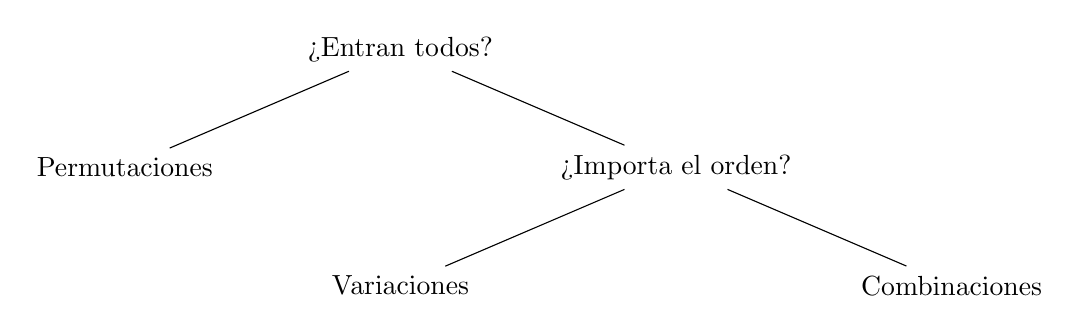
\begin{tikzpicture}[sibling distance=70mm]
		\node {¿Entran todos?}
		child {node {Permutaciones}}
		child {node {¿Importa el orden?}
		child {node {Variaciones}}
		child {node {Combinaciones}}
		};
	\end{tikzpicture}
\end{center}

\begin{tabular}{c|c|c}
	Permutaciones & Variaciones & Combinaciones \\
	\hline
	\begin{tabular}{c|c}
		Sin    & Con \\
		$\text{P}_n = n!$ & $\text{PR}^n_{n_1,\cdots,n_k}=\frac{n!}{n_1!\cdots n_k!}$
	\end{tabular} & \begin{tabular}{c|c}
		                Sin                      & Con \\
		                $\text{V}^n_p = \frac{n!}{(n-p)!}$ & $\text{VR}^n_p = n^p$
	\end{tabular} & \begin{tabular}{c|c}
		                Sin                & Con  \\
		                $\text{CR}^n_p =  \binom{n}{p}$ & $\text{C}^n_p = \binom{n+p-1}{p}$
	\end{tabular}
\end{tabular}

\subsection{Variaciones}

\begin{example}
	¿Cuántas banderas diferentes de tres franjas horizontales de colores distintos pueden confeccionarse a
	partir de siete colores diferentes?

	Tenemos un conjunto $C$ de $n=7$ colores distintos, y por tanto distinguibles, y queremos elegirlos para formar elementos de $C^3$, el número de elementos distintos es
	\[
		\text{V}^7_3=\frac{7!}{(7-3)!}=\frac{7!}{4!}=7*6*5=210
	\]
\end{example}

\begin{example}
	¿Cuántas quinielas de 14 resultados distintas se pueden rellenar?

	Tenemos un conjunto $C=\set{1, x, 2}$ de $n=3$ elementos y tenemos que formar elementos de $C^{14}$.
	\[
		\text{VR}^{3}_{14} = 3^{14}=4782969
	\]
\end{example}

\subsubsection{Permutaciones con repetición}
Podemos formar $k$ grupos indistinguibles de cardinales $n_1,\cdots, n_k\tq \sum_{i=1}^k n_i=n$.


\begin{example}
	¿Cuántos números de seis cifras se pueden formar con los dı́gitos 1, 2 y 3?

	Se trata de determinar el número de ordenaciones distintas de un conjunto de seis elementos formados por tres
	grupos distintos de elementos indistinguibles, $\set{1, 1, 1}, \set{2, 2}, \set{3}$.
	\[
		\text{PR}^6_{3,2,1}=\frac{6!}{3! 2! 1!}=60
	\]
\end{example}

\subsection{Combinaciones}

\begin{example}
	Un estudiante debe responder a seis de las diez preguntas de las que consta un examen, ¿cuantas formas distintas tiene de hacer el examen?

	Se trata de determinar el número de grupos distintos de seis preguntas escogidas del conjunto de las diez, sabiendo que dos grupos con las mismas preguntas, aún en distinto orden, coinciden.
	En este caso, el número de grupos de preguntas distintos entre los que se puede elegir es
	\[
		\text{C}^{10}_6 = \begin{pmatrix*}
			                  10\\6
		\end{pmatrix*} =\frac{10!}{6!(10-6)!}=\frac{10!}{6!4!}=\frac{10*9*9*7}{4*3*2}=210
	\]
\end{example}

\begin{example}
	¿De cuántas formas pueden elegirse simultáneamente tres bolas de una urna en la que hay al menos tres bolas bolas blancas y tres negras indistinguibles?

	Cada grupo es una disposición no ordenada de tres colores formada por los colores blanco y negro con repetición de alguno de ellos.
	Por tanto, se trata de determinar el número de grupos de tres elementos no ordenados del conjunto {b, n}.
	En este caso, el número de formas distintas de elegir simultáneamente tres bolas del conjunto es
	\[
		\text{CR}^2_3=\begin{pmatrix*}
			              4\\3
		\end{pmatrix*} =\frac{4!}{3!1!}=4
	\]
\end{example}
	\section{Códigos perfectos}

Sobre $\Z_q^n$, como extensión de las operaciones sobre $Z_q$ podemos definir las operaciones : $\forall x, y\in\Z_q^n$
\begin{align*}
	x\mas y &= x_1\mas y_1\cdots x_n\mas y_n\\
	x\menos y &= x\mas (-y)\\
	x\por y &= x_1\por y_1\cdots x_n\por y_n
\end{align*}

\begin{definition}
	Sea $x$ una palabra de longitud $n$, definimos el \define{soporte}{soporte} de $x$ como $sop(x)=\set{i\tq x_i\neq 0, i=1,\dots, n}$.
\end{definition}

\begin{definition}
	Sea $x$ una palabra de longitud $n$, se define el \define{peso}{peso} de $x$ a $w(x)=|sop(x)|$.
\end{definition}
\begin{lemma}
	\label{res:distancia-peso}
	Sean $x, y$ dos palabras de longitud $n$, se tienen los siguientes resultados:
	\begin{enumerate}
		\item $w(x) = d(\vec{0},x)\so w(x)=n-\sum_{i=1}^n \delta_{0x_i}$.
		\item $d(x,y)=w(x\menos y)$.
		\item Si $q$ es primo, $w(x\menos y)=w(x)+w(y)-2w(x\por y)$.
	\end{enumerate}
\end{lemma}

\begin{lemma}
	Sean $q, n, k, d\in\N$ con $d$ impar y $q$ primo.\ Existe $C$ un $(q, n, k, d)$-código con $q$ primo si y sólo si existe $C'$ un $(q, n+1, k, d+1)$-código.
\end{lemma}
\begin{proof}
	$\so$) Dado $C=\set{x_1, \dots, x_k}$ un $(q, n, k, d)$-código, podemos construir $C'=\set{y_1,\dots, y_k}$ un $(q, n+1, k, d+1)$-código binario definiendo

	\[
		y_i=\begin{cases}
			    x_{i1}\cdots x_{in}0 & \text{ si $w(x_i)$ es par}\\
			    x_{i1}\dots x_{in}1 & \text{ si $w(x_i)$ es impar}
		\end{cases}
	\]
	Por construcción se tiene que $w(y_i)$ siempre es par y por tanto se tendrá también que $d(y_i, y_j)$ es par pues
	\[
		d(y_i, y_j) = w(y_i) + w(y_j) - 2 w(y_i\por y_j)
	\]
	Por lo tanto $r(C')$ es par.\ Por otra parte se tiene que
	\begin{align*}
		d(y_i, y_j) = d(x_i, x_j)+\delta_{x_{in+1}x_{jn+1}}\so d(y_i, y_j)\geq d(x_i, x_j) \so r(C')\geq r(C)
	\end{align*}
	Como $d=r(C)$ es impar, la desigualdad es estricta, pero como existen al menos dos palabras clave $x_l, x_m$ tal que $d(x_l, x_m) = d$, tenemos que $d(y_l, y_m) = d+1$ alcanzando la igualdad buscada.

	$\Leftarrow$) Para el recíproco sea $C$ un $(q, n+1, k, d+1)$-código y dos palabras clave $x_l$ y $x_m$ de $C$  para las cuales $d(x_l, x_m) = d+1$, sea $i$ un índice donde $x_{li}\neq x_{mi}$, y por permutación llevemos $C$ a otro código equivalente, y por tanto con el mismo radio interior, para que $i=n+1$.

	Se construye $C'=\set{y_1,\dots y_k}$ de la siguiente forma
	\[
		y_i = x_{i1}\dots x_{in}
	\]
	Con el mismo desarrollo que arriba se tiene que $d(y_i, y_j) < d(x_i, x_j)$ con lo que $r(C')< r(C)$ y para comprobar que se alcanza la igualdad buscada tenemos que $d(y_l, y_k) = d(x_l, x_k)-1=d+1-1=d$.
\end{proof}

\begin{theorem}[Sphere-packing o Hamming bound]
	Un $(q, n, M, 2t+1)$-código satisface $M|B(0, t)|\leq 2^n$.
\end{theorem}

\begin{definition}
	Diremos que un $(q, n, M, 2t+1)$-código es un \define{código perfecto}{codigo_perfecto} si $M|B(0, t)|= 2^n$.
\end{definition}

Para buscar códigos perfectos no triviales, vamos a centrarnos en una familia de códigos llamados de bloques con diseños balanceados.

\subsection{Códigos de bloques con diseños balanceados}
\begin{definition}
Un \define{bloque con diseño balanceado}{bloque-diseño-balanceado} es un conjunto $S$ de $v$ elementos, llamados puntos, una colección de $b$ subconjuntos de $S$ llamados bloques y 3 valores $k, r$ y $\lambda$ tal que
	\begin{enumerate}
		\item Cada bloque contiene exactamente $k$ puntos.
		\item Cada punto pertenece a $r$ bloques.
		\item Cada par de puntos están juntos en $r$ bloques.
	\end{enumerate}
	Un código de estas características de denota un $(b, v, r, k, \lambda)$-diseño.
\end{definition}

\begin{example}
	Toma $S=\set{1, 2, 3, 4, 5, 6, 7}$ y los siguientes subconjuntos $S_1=\set{1, 2, 4}, S_2=\set{2, 3, 5}, S_3=\set{3, 4, 6}, S_4=\set{4, 5, 7}, S_5=\set{5, 6, 1}, S_6=\set{6, 7, 2}$ y $S_7=\set{7, 1, 3}$.
	\[
		\begin{tabular}{c|ccccccc}
			& 1 & 2 & 3 & 4 & 5 & 6 & 7\\
			\hline
			1& 3 & 1 & 1 & 1 & 1 & 1 & 1\\
			2& 1 & 3 & 1 & 1 & 1 & 1 & 1\\
			3& 1 & 1 & 3 & 1 & 1 & 1 & 1\\
			4& 1 & 1 & 1 & 3 & 1 & 1 & 1\\
			5& 1 & 1 & 1 & 1 & 3 & 1 & 1\\
			6& 1 & 1 & 1 & 1 & 1 & 3 & 1\\
			7& 1 & 1 & 1 & 1 & 1 & 1 & 3
		\end{tabular}
		\qquad
		\begin{tabular}{c|ccccccc}
			& $S_1$ & $S_2$ & $S_3$ & $S_4$ & $S_5$ & $S_6$ & $S_7$\\
			\hline
			1& 1 & 0 & 0 & 0 & 1 & 0 & 1\\
			2& 1 & 1 & 0 & 0 & 0 & 1 & 0\\
			3& 0 & 1 & 1 & 0 & 0 & 0 & 1\\
			4& 1 & 0 & 1 & 1 & 0 & 0 & 0\\
			5& 0 & 1 & 0 & 1 & 1 & 0 & 0\\
			6& 0 & 0 & 1 & 0 & 1 & 1 & 0\\
			7& 0 & 0 & 0 & 1 & 0 & 1 & 1
		\end{tabular}
	\]
	La primera tabla muestra en cuantos subconjuntos está incluido el conjunto $\set{i,j}$ y la segunda tabla muestra a qué conjunto pertenece $i$, visto como matrices tendríamos dos matrices $A=(a_{ij})$ y $B=(b_{ij})$ definidas por
	\begin{align*}
		a_{ij} & =|\set{k\tq \set{i,j}\subseteq S_k}|\\
		b_{ij} & =|\set{i}\cap S_j|
	\end{align*}
	La matriz $A$ nos permite comprobar los puntos 2 y 3 de la definición anterior y la matriz $B$ nos permite comprobar los puntos 1 y 2, con lo cual podemos ver que tenemos un $(7, 7, 3, 3, 1)$-diseño.
\end{example}

\begin{definition}
	Sea un $(b, v, r, k, \lambda)$-diseño, con bloques $B_1,\dots, B_v$.
	Definimos la \define{matriz de incidencia}{matriz-incidencia} de $C$ a la matriz $A=(a_{ij})\in M_{v\times b}(\Z_2)$ definida por $a_{ij} = |\set{i}\cap B_j|$.
\end{definition}

\begin{example}
	Volviendo al ejemplo anterior, consideremos el conjunto $C=\set{\logical{0}{7}, \logical{1}{7}}\cup \set{a_i}_{i=1}^7\cup \set{b_i}_{i=1}^7$ donde $a_i$ son las filas de la matriz incidencia $B$ y $b_i = -a_i$.
	Esta construcción nos permite tener un $(7, 16 ,3)$-código perfecto
\end{example}

\begin{lemma}
	Sea un $(b, v, r, k, \lambda)$-diseño.\ Se cumple:
	\begin{itemize}
		\item $bk=vr$.
		\item $r(k-1)=\lambda(v-1)$.
		\item $v\leq b$.
	\end{itemize}
\end{lemma}

\begin{definition}
	Un $(b, v, r, k, \lambda)$-diseño es un \define{diseño simétrico}{diseño-simetrico} si $b=v$.
	Por el resultado anterior, se tendrá también que $k=r$ y por tanto podemos denotar a estos diseños como un $(v, k, \lambda)$-diseño.
\end{definition}
	\section{Códigos lineales}
A lo largo de este capítulo consideramos que el alfabeto $\Gamma$ es el cuerpo de Galois $GF(q)$ donde $q$ es una potencia de un primo y que $\Gamma^n$ es el espacio vectorial $V(n, q)$.
\begin{definition}
	Un código de $GF(q)$ se dice que es un \define{código lineal}{codigo-lineal} si es un subespacio vectorial de $V(n, q)$ para algún $n\in\N$.
	Si $C$ es un código lineal de $V(n, q)$ de dimensión $k$ y radio interior $d$, diremos que $C$ es un $[q, n, k, d]$-código o un $[q, n, k]$-código.
\end{definition}
Observaremos que un $[q, n, k, d]$-código es un $(q, n, q^k, d)$-código y que dado dos palabras claves, su diferencia también es una palabra clave, obliga a que $\vec{0}$ sea también una palabra clave y junto con el resultado~\ref{res:distancia-peso}, obtenemos el siguiente resultado.
\begin{lemma}
	\label{res:distancia-peso-lineal}
	Para todo código lineal $C$ existe $x\in C$ tal que $r(C)=w(x)=\min\set{d(\vec{0}, a)\ \forall a\in C}$.
\end{lemma}

\subsection{Matriz generador}
Sea $C$ un código lineal, como subespacio vectorial finito, tenemos una base por el cual todo elemento de $C$ es combinación lineal, y asociada a esta base tenemos una matriz, que nos permite identificar códigos equivalentes con matrices equivalentes en el sentido que veremos más adelante.

\begin{definition}
	Sea $C$ un $[q, n, k]$-código lineal, dada una base $B=\set{\lista{x_1}{x_k}}$ llamaremos matriz generadora de $C$ asociada a $B$ a la matriz $X=(x_{ij})\in M_{k\times n}(GF(q))$.
\end{definition}
Como vemos por la definición, un código lineal tiene tantas matrices generadoras como bases distintas, por eso es conveniente establecer características que nos permitan saber cuando distintas matrices generan el mismo código o código equivalentes.
\begin{example}
	\label{ex:matriz-generador}
	Consideremos el código $C$ formado por las siguientes palabras de $\Z_2^7$
	\begin{align*}
		\vec{0} & \ & \vec{1} & \ \\
		x_1 &= 1000101 & y_1 &= 0111010\\
		x_2 &= 1100010 & y_2 &= 0011101\\
		x_3 &= 0110001 & y_3 &= 1001110\\
		x_4 &= 1011000 & y_4 &= 0100111\\
		x_5 &= 0101100 & y_5 &= 1010011\\
		x_6 &= 0010110 & y_6 &= 1101001\\
		x_7 &= 0001011 & y_7 &= 1110100
	\end{align*}
	Para calcular el radio interior de $C$ por el resultado~\eqref{res:distancia-peso-lineal} simplemente tenemos que calcular los pesos de cada elemento
	\begin{align*}
		w(0) &= 0 & w(1) &= 7 \\
		w(x_1) &= 3 & w(y_1) &= 4 \\
		w(x_2) &= 3 & w(y_2) &= 4 \\
		w(x_3) &= 3 & w(y_3) &= 4 \\
		w(x_4) &= 3 & w(y_4) &= 4 \\
		w(x_5) &= 3 & w(y_5) &= 4 \\
		w(x_6) &= 3 & w(y_6) &= 4 \\
		w(x_7) &= 3 & w(y_7) &= 4 \\
	\end{align*}
	Así que $C$ es un $(2, 7, 16, 3)$-código que también es un $[2, 7, 4, 3]$-código lineal.
	Para buscar una base de $C$ observemos que
	\begin{align*}
		y_i &= \vec{1}+x_i\ \forall i=1,\dots, 7\\
		x_4 &= \vec{1}+x_1+x_2\\
		x_5 &= \vec{1}+x_2+x_3\\
		x_6 &= x_1+x_2+x_3\\
		x_7 &= \vec{1}+x_1+x_3
	\end{align*}
	Por tanto $B=\set{\vec{1}, x_1, x_2, x_3}$ es una base de $C$ que tiene como matriz asociada a
	\[
		X=\begin{pmatrix*}
			  1&1&1&1&1&1&1\\
			  1&0&0&0&1&0&1\\
			  1&1&0&0&0&1&0\\
			  0&1&1&0&0&0&1
		\end{pmatrix*}\in M_{4\times 7}(\Z_2)
	\]
\end{example}

\subsection{Código lineales equivalentes}
Para código lineales, vamos a modificar ligeramente la definición de códigos equivalentes que se dio en~\eqref{def:codigo-equivalente} pues tomando la misma relación de equivalencia, sólo vamos a restringir las transmutaciones válidas a las traslaciones no nulas sobre un índice, es decir, para las que exista $\lambda\neq 0\in GF(q)$ y $\maps{T_{i\lambda}}{V(n, q)}{V(n, q)}$ a la aplicación definida por
\[
	T_{i\lambda}(\palabraG)=y_1\cdots y_n \text{ donde } y_k = \begin{cases}
		                                                            \lambda x_i \text{ si } k = i \\
		                                                            x_k \text{ resto}
	\end{cases}
\]

Lo que estamos buscando con esta definición es obtener transformaciones de códigos lineales que conlleven asociadas matrices que generen las mismas ecuaciones como generadores, y como recordaremos, cuando se resuelven ecuaciones lineales, al trabajar con la matriz asociada teníamos permitidos los siguientes operaciones
\begin{itemize}
	\item[R1] $\Rr{i}{j}$ Permutación de filas.
	\item[R2] $\Rrr{i}{\lambda}$ Multiplicación de fila por escalar no nulo.
	\item[R3] $\Rrrr{i}{j}{\lambda}$ Cambio de una fila por el resultado de suma por otra fila multiplicada por un escalar no nulo.
	\item[C1] $\Cc{i}{j}$Permutación de columnas.
	\item[C2] $\Ccc{i}{\lambda}$ Multiplicación de columna por escalar no nulo.
\end{itemize}

\begin{example}
	En el ejemplo~\eqref{ex:matriz-generador} hemos cogido las palabras clave $\vec{1}, x_1, x_2, x_3$ como base de $C$ pero podríamos perfectamente haber considerado como base las palabras clave $\vec{1}, x_3, x_4, x_5$ con lo que hubiéramos obtenido la matriz generadora
	\[
		Y=\begin{pmatrix*}
			  1&1&1&1&1&1&1\\
			  0&1&1&0&0&0&1\\
			  1&0&1&1&0&0&0\\
			  0&1&0&1&1&0&0
		\end{pmatrix*}
	\]
	Veamos como obtener la matriz $Y$ a partir de la $X$ con las operaciones R1, R2, R3, C1 y C2.
	\begin{align*}
		X&=\begin{pmatrix*}
			   1&1&1&1&1&1&1\\
			   1&0&0&0&1&0&1\\
			   1&1&0&0&0&1&0\\
			   0&1&1&0&0&0&1
		\end{pmatrix*}\Rr{2}{4}
		\begin{pmatrix*}
			1&1&1&1&1&1&1\\
			0&1&1&0&0&0&1\\
			1&1&0&0&0&1&0\\
			1&0&0&0&1&0&1
		\end{pmatrix*}\Rrrr{4}{3}{1}
		\begin{pmatrix*}
			1&1&1&1&1&1&1\\
			0&1&1&0&0&0&1\\
			1&1&0&0&0&1&0\\
			0&1&0&0&1&1&1
		\end{pmatrix*}\Rrrr{4}{1}{1}\\
		&\Rrrr{4}{1}{1}
		\begin{pmatrix*}
			1&1&1&1&1&1&1\\
			0&1&1&0&0&0&1\\
			1&1&0&0&0&1&0\\
			1&0&1&1&0&0&0
		\end{pmatrix*}\Rr{4}{3}
		\begin{pmatrix*}
			1&1&1&1&1&1&1\\
			0&1&1&0&0&0&1\\
			1&0&1&1&0&0&0\\
			1&1&0&0&0&1&0
		\end{pmatrix*}\Rrrr{4}{2}{1}
		\begin{pmatrix*}
			1&1&1&1&1&1&1\\
			0&1&1&0&0&0&1\\
			1&0&1&1&0&0&0\\
			1&0&1&0&0&1&1
		\end{pmatrix*}\Rrrr{4}{1}{1}\\
		&\Rrrr{4}{1}{1}
		\begin{pmatrix*}
			  1&1&1&1&1&1&1\\
			  1&0&1&1&0&0&0\\
			  0&1&0&1&1&0&0\\
			  0&1&0&1&1&0&0
		\end{pmatrix*}=Y
	\end{align*}

\end{example}
	\section{Codificando y decodificando con códigos lineales}
Sea $C$ un $[q, n, k, d]$-código lineal con matriz generadora $G$, todo elemento $x=\palabraG\in C$ se puede poner de la forma $x=yG$ para algún $y\in\Z_q^k$, podemos identificar cada palabra clave de $C$ con un elemento de $\Z_q^k$ y obviamente al revés también, por la propia definición de generador, podemos considerar un isomorfismo entre $C$ y $\Z_q^k$.

\begin{definition}
	Sea $C$ un $[q, n, k, d]$-código lineal con matriz generadora $G$, llamaremos \define{codificación}{codificacion} de $C$ al isomorfismo $\maps{d}{Z_q^k}{C}$ definido por $d(y)=yG$.\ Al isomorfismo inverso lo llamaremos \define{decodificación}{decodificación} de $C$.
\end{definition}

\subsection{Codificación}
Vamos a definir un tipo muy especial, mediante las operaciones R1, R2, R3, C1 y C2 podemos transformar al matriz generadora $G$ en otra equivalente de la forma $[I_k|G']$ donde $G'\in M_{k\times (n-k)}(\Z_q)$, y con esta matriz observamos que dado $y=\palabraN{y}$ la palabra clave en $C$ viene dado por $x=y[I_k|G']$ y por lo tanto
\begin{align*}
	x_i &= \sum_{j=1}^k y_j [I_k|G']_{ji}=\begin{cases}
		                                     \sum\limits_{j=1}^k y_j (I_k)_{ji}=y_i \text{ si $1\leq i \leq k$} \\
		                                     \sum\limits_{j=1}^k y_j G'_{jk} \text{ si $i > k$}
	\end{cases}
\end{align*}
Obtenemos así que las palabras $y$ en $\Z_q^k$ se convierten en palabras clave de la forma $yy'$ en $\Z_q^n$ donde $y'\in\Z_q^{n-k}$.

\begin{definition}
	Sea $C$ un $[q, n, k]$-código lineal con matriz generadora $G$.\ Diremos que la matriz está en su \define{forma estándar}{matriz-forma-estandar} si $G=[I_k|G']$ con $G'\in M_{k\times (n-k)}(\Z_q)$.
\end{definition}

\begin{definition}
	Sea $C$ un $[q, n, k]$-código lineal con matriz generadora $G=[I_k|G']$ en su forma estándar, a la palabra $yG'$ donde $y\in \Z_q^{n-k}$ se la llamamos \define{palabra de control}{palabra-control}.
	A la matriz $G'$ la llamamos \define{matriz de control}{matriz-control}.
\end{definition}

Esta manera de codificar nos permite acceder a la información que hemos codificados y además, las palabras de control nos añade una protección adicional ante fallos en la codificación.

\begin{example}
	Siguiendo con el ejemplo~\ref{ex:matriz-generador}, es sencillo encontrar que una matriz generadora de $C$ en su forma estándar es
	\[
		G=\begin{pmatrix*}
				1&0&0&0&1&0&1\\
				0&1&0&0&1&1&1\\
				0&0&1&0&1&1&0\\
				0&0&0&1&0&1&1
		\end{pmatrix*}
	\]
	La matriz de control es
	\[
		G'=\begin{pmatrix*}
			  1&0&1\\
			  1&1&1\\
			  1&1&0\\
			  0&1&1
		\end{pmatrix*}
	\]
	Y la codificación de la palabra $y=1110$ nos genera la palabra de control $y'=100$ y por tanto obteniendo la palabra clave $x=1110100$.
\end{example}

\subsection{Decodificación}
Recordemos del primer capítulo que al recibir una palabra que no estuviera en el código $C$, hay que averiguar si el error producido era recuperable, y que esta situación se daba cuando la distancia de la palabra recibida a $C$ era menor o igual al grado de corrección de $C$.

Cuando trabajamos con código lineales, si $x\in C$ es la palabra clave enviada y $\push{x}$ la palabra recibida, tenemos que

\begin{equation}
	\label{eq:distancia-recibida-codigo-lineal}
	d(\push{x}, C) = \min_{y\in C}\set{d(\push{x}, y)}= \min_{y\in C}\set{w(\push{x}\menos y)}=w(\push{x}\menos C)
\end{equation}

Veamos con un poco más de detalle los conjuntos $y\menos C$ o lo que es lo mismo $y\mas C$.
\begin{definition}
	Sea $C$ un código lineal y $a\in V(q, n)$.\ Definimos el \define{coset}{coset} de $C$ en $a$ a
	\[
		a+C=\set{a\mas x\ \forall x\in C}
	\]
\end{definition}
\begin{lemma}
	Sea $C$ un código lineal y $a, b\in V(q, n)$.\ Se cumple que
	\begin{itemize}
		\item $a+C = b+C\iff a\menos b\in C$.
		\item $(a+C) \cap (b+C) = \emptyset \iff a\menos b\notin C$.
	\end{itemize}
\end{lemma}

\begin{lemma}
Sea $C$ un $[q, n, k, d]$-código lineal.\ Existen $a_1, \dots, a_s$ elementos de $V(q, n)$ donde $s=q^{n-k}$ tal que $V(q,n)$ es unión disjunta de la forma
	\[
		V(n, q) = (a_1+C)\cup\dots\cup (a_s+C)
	\]
\end{lemma}

Todos los conjuntos de la forma $x+C$ tienen exactamente $q^k$ elementos, uno de ellos es el propio $C$, con lo que podemos considerar $a_1=\vec{0}$.\ Pero no nos interesa cualquier partición en cosets de $V(q, n)$, sino aquellos que nos digan rápidamente a que palabra clave están más próximos, y por~\eqref{eq:distancia-recibida-codigo-lineal} de cada coset nos quedamos como representante aquel que tenga el peso más bajo.

\begin{definition}
	Sea $C$ un código lineal y $a\in V(q, n)$.\ Definimos el \define{coset}{coset} de $C$ en $a$ a
\end{definition}
	\section{Ruido en el canal}
Ahora vamos a tratar estudiar el caso de comunicación con ruido, desde un punto de vista probabilístico.\ Vamos a considerar códigos binarios ($q=2$) y que la probabilidad de que se genere un error es $p$ con independencia del símbolo transmitido, que llamaremos un canal binario y simétrico de error $p$.

La probabilidad de recibir una palabra de $n$ símbolos tenga exactamente $k$ errores es $\binom{n}{k}p^k(1-p)^{n-k}$ y si $C$ es un código de radio interior $d$, la probabilidad de que la palabra recibida sea correctamente corregida es que haya sufrido menos o igual a $s$ errores es $\sum_{k=0}^s \binom{n}{k} p^k(1-p)^{n-k}$ donde $s$ es el grado de corrección de $C$.

Denotaremos por $P_{corr}(C)$ la probabilidad de la correcta corrección de palabras de un código y por $P_{err}(C)$ a la probabilidad de error en la corrección.
\[
	P_{corr}(C) = \sum_{k=0}^s \binom{n}{k} p^k(1-p)^{n-k}=(1-p)^{n-s}\sum_{k=0}^s \binom{n}{k} p^k(1-p)^{s-k}
\]

Esta expresión nos permite ver que para cualquier canal con ruido, podemos usar códigos con longitudes de palabras $n$ tan grandes como queramos para que la probabilidad de corrección sea tan grade como queramos.\ Sin embargo, no podemos saturar el canal con cualquier longitud, pues el canal tiene una capacidad de transmisión, tenemos que calcular y saber obtener el código cuya longitud y grado de corrección permita una correcta transmisión/corrección.

Recordemos que para un canal de transmisión con ruido definido por una variable de probabilidad aleatoria $X$ con probabilidades $p_x=P(X=x)$, se define la \define{entropía de Shannon}{entropia-shannon} por $H(X)=\sum_{x\in X}p_x \log_2(p_x)$~\cite{shannon}.
En este contexto, la entropía de Shannon es $H(X)=p \log_2(p) + (1-p) \log_2(1-p)$.

\begin{definition}
	Llamamos \define{capacidad}{capacidad} $C(p)$ de un canal binario y simétrico $F$ a $C(F)=1+H(F)$.
\end{definition}

Terminamos el capítulo recordando el teorema de Shannon
\begin{lemma}
	Sea $F$ un canal binario y simétrico de error $p$ y $R$ un valor menor que la capacidad de $F$.\ Para todo $\epsilon>0$ existe un valor de $n$ y un $[2, n, k]$-código tal que $k/n\geq R$ y $P_{err}(C)<\epsilon$.
\end{lemma}
	\section{Códigos ortogonales}
Recordemos que el producto interno sobre $\Z_q^n$ se define por
\[
	x\cdot y=\sum_{i=1}^n x_i y_i\mod q
\]
y que dado un conjunto $X\subset \Z_q^n$ definimos el conjunto ortogonal $X^\perp$ por
\[
	X^{\perp}=\set{y\in\Z_q^n\tq y\cdot x = 0\ \forall x\in X}
\]
que por las propiedades del producto interno hacen del conjunto ortogonal un subespacio vectorial.

Para códigos lineales $C$, tomando una matriz generadora $G=(g_{ij})$ los elementos $y=\palabraN{y}$ de $C^\perp$ tienen que satisfacer las ecuaciones
\[
	\sum_{j=1}^n g_{ij}y_j=0\ \forall i=1,\dots, k
\]
que nos permite obtener $n-k$ soluciones linealmente independientes, por lo tanto $\dim(C^\perp)= n-\dim(C)$.

Decir que $C\cdot C^\perp=0\so C\subseteq (C^\perp)^\perp$ y por tanto
\[
	\dim(C)\leq \dim((C^\perp)^\perp)= n-dim(C^\perp)= n-(n-dim(C))=\dim(C)\so C=(C^\perp)^\perp
\]
Juntando todos estos resultados obtenemos el siguiente resultado
\begin{lemma}
	Sea $C$ un $[q, n, k]$-código.\ Se tiene que $C^\perp$ es un $[q, n, n-k]$-código.
\end{lemma}

\subsection{Matriz de paridad}
Dado un código lineal $C$ con matriz generadora $G$, tenemos que $C^\perp$ es también un código lineal y por tanto también podemos obtener una matriz generadora $H$ que por definición cumple $GH^T=0$.
Ya que decir que $C^\perp$ es ortogonal a $C$ es lo mismo que decir que $C$ es ortogonal a $C^\perp$, lo mismo da tener $G$ que $H$ para tener definidos ambos códigos.

\begin{definition}
	Sea $C$ código lineal.\ Llamamos \define{matriz de paridad}{matriz-paridad} de $C$ a la matriz generadora de $C^\perp$.
\end{definition}

Podemos obtener la siguiente relación entre ambas matrices
\[
	G=[I_k|A]\so H=[-A^T|I_{n-k}]
\]

\begin{definition}
	Sea $C$ código lineal.\ Diremos que $H$ la matriz de paridad está en su \define{forma estándar}{matriz-paridad-forma-estandar} si está en la forma $H=[B|I_{n-k}]$.
\end{definition}

Siguiendo con el ejemplo~\ref{ex:matriz-generador}, cuya matriz generadora en su forma estándar es
\[
	G=\begin{pmatrix*}
		  1&0&0&0&1&0&1\\
		  0&1&0&0&1&1&1\\
		  0&0&1&0&1&1&0\\
		  0&0&0&1&0&1&1
	\end{pmatrix*}
\]
Tiene por tanto la matriz de paridad
\[
	H=\begin{pmatrix*}
		  1&1&1&0&1&0&0\\
		  0&1&1&1&0&1&0\\
		  1&1&0&1&0&0&1\\
	\end{pmatrix*}
\]
	\printbibliography
\end{document}